\documentclass[main]{subfiles}


\begin{document}
\newpage
\section{Plasticity In The Brain}

%---------------------------
\subsection{Why do we need plasticity?}
Why this topic is relevant:
\begin{itemize}
    \item Biological plasticity might provide a different angle to understand the training procedures in DNNs.
    \item Given the effectiveness of human brain learning bio-plasticity might provide inspiration/new ideas for improved DNN training algorithms. Example: the idea of drop out (in DNNs the network randomly get rid of single neurons to prevent too much information to be stored in single neurons and weights. This was observed in neuroscience first)
    \item Understanding biological plasticity might help to better understand how (hierarchical) learning is organized in the brain (Learning and Memory).
    \item Many neural disorders such as dementia might relate to a disturbance in neuronal plasticity that cause neuronal networks to become dysfunctional. Some plasticity mechanisms /disorders lead to malfunction in the brain.
    \item All intelligent behavior is learned so we need plasticity to learn. 
    \item The brain a universal learning machine, some information is genetically present at birth such as babies ability to distinguish faces but the rest is learned thus requires plasticity. 
\end{itemize}
\begin{itemize}
    \item[\textbf{Plasticity}] Allows acquisition of knowledge/information and the formation of memory through experience
    \item[\textbf{Memory}] Storage of information that can be recalled later. Learning results in memory - which has further outcome - it can change future behavior
    \item[\textbf{Learning Curve}] Training to do tasks or reacting to stimuli, at the beginning bad and over the course of a few days vastly improves
\end{itemize}
%
Everything we do is \textit{learning} and for that we need \textit{plasticity}. An illustrative example below\footnote{Kandel, \textit{Principles of neural science}, 2001}, according to the motto: "Here I get a reward, here not".
%
\begin{figure}[H]
    \centering
    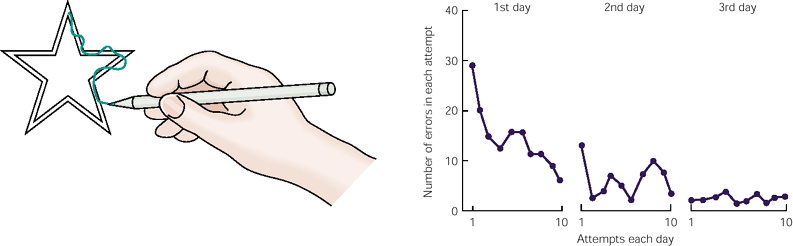
\includegraphics[width=\textwidth]{03_PlasticityInTheBrain/figures/motorlearning.jpg}
    \caption{Motor learning task. Some human subjects have got the task to draw. Having gotten an (electrical) feedback, this subjects learned the pattern they had to draw}
    \label{fig:motorlearning}
\end{figure}

%---------------------------
\subsection{Synaptic Plasticity}

\subsubsection{Biological Recap}
In synaptic plasticity one understands changes in reactivity of \textbf{post}- to \textbf{pre}synaptic neuron. In other words, plasticity changes of chemical synapses can strengthen or weaken transmission. This changes can last from milliseconds (short-term) to weeks or longer (long-term).
\begin{itemize}
    \item[\textbf{EPSP}] Excitatory postsynaptic potential
    \item[\textbf{LTP}] long term potentiation; long lasting increase in synaptic strength, i.e. EPSP amplitude. Through more AMPA receptors and more released vesicles per action potential, the neuron depolarizes more after recieving an AP.
    \item[\textbf{LTD}] long term depression; long lasting decreaes in synaptic strength; neurons do not depolarize as much. 
    \item[\textbf{Glutamate}] Neurotransmitter leading to excitability depolarization
    \item[\textbf{GABA}] Neurotransmitter leading to inhibition hyperpolarization
\end{itemize}

\paragraph{Recap of Synaptic Plasticity} (\textit{see} Figure \ref{fig:syn_plast}):
\begin{enumerate}
    \item Action potential (AP) comes down the axon of neuron 1, this causes a change in  voltage (depolarisation)
    \item \ce{Ca^2+} channels open, \ce{Ca^2+} influx
    \item Neurotransmitters (NT) get released
    \item NT cross synaptic cleft and bind to the dendrite of neuron
    \item bind to postsynaptic receptors (e.g. AMPA receptors), which increases the depolarisation probability.
\end{enumerate}

\begin{figure}[H]
    \centering
    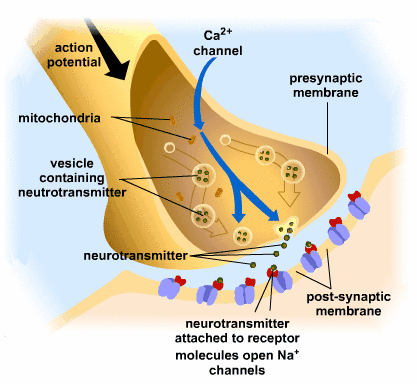
\includegraphics[width=.6\textwidth]{03_PlasticityInTheBrain/figures/synaptic_plasticity.jpg}
    \caption{Pre- and post-synaptic neuron}
    \label{fig:syn_plast}
\end{figure}


\paragraph{Synaptic Plasticity Alters the interneuron Connection Strength:} As the Amplitude of the EPSP increase it leads to a change in the producing and  receiving neuron. This allows the neuron to scale up or down in response to the received activity. In the short term the AMPA / NMDA channels increase, synaptic density size changes, in the long term (around 30 minutes) the number of spines increase thus creating more synapses 

\begin{figure}[H]
    \centering
    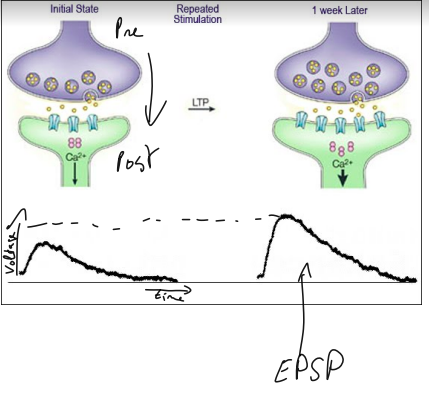
\includegraphics[width=.6\textwidth]{03_PlasticityInTheBrain/figures/pasted_image_1.png}
    \caption{}
    \label{fig:syn_plast1}
\end{figure}

\begin{figure}[H]
    \centering
    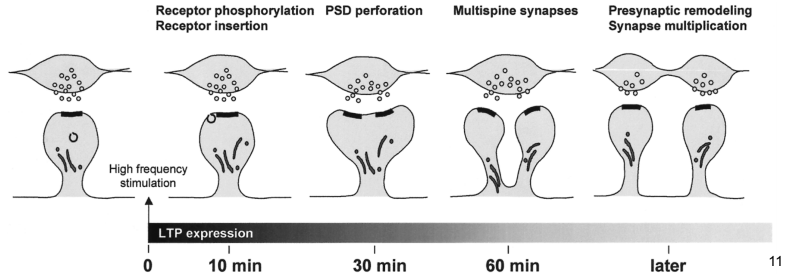
\includegraphics[width=.8\textwidth]{03_PlasticityInTheBrain/figures/pasted_image_2.png}
    \caption{}
    \label{fig:syn_plast1}
\end{figure}


\subsubsection{Homeostatic Plasticity}
The cells want to keep a steady firing rate so it turns the excitability of the synapses. This is called Synaptic scaling is the global activity the cell wants to keep, either increasing/decreasing the average activity level. It is not synaptic specific. 

Example: isolated neurons are given inhibitors or excitatory chemical. Then washed the chemical effects off and the neuronal activity will spike in the inhibitory neurons and decrease in the artificially excited neurons. 

When information is propagated through a heircal network you want a certain amount of information expressed at each layer this prevent loss or explosion of information. This is similar to what occurs in deep networks, batch normalisation and weight decay, you want a certain activativation so that there is not uniform de/activation in the layers 

\begin{figure}[H]
    \centering
    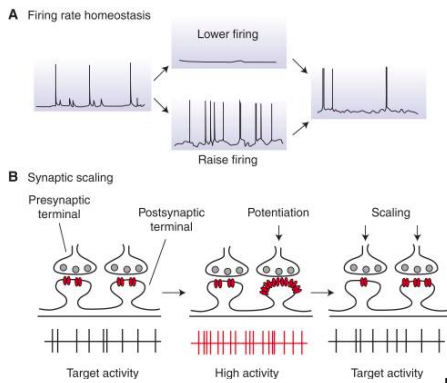
\includegraphics[width=.7\textwidth]{03_PlasticityInTheBrain/figures/pasted_image_4.png}
    \caption{Pre- and post-synaptic neuron}
    \label{fig:syn_plas1t}
\end{figure}

\begin{figure}[H]
    \centering
    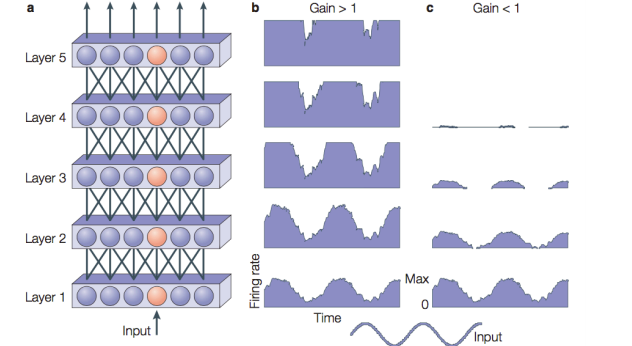
\includegraphics[width=.7\textwidth]{03_PlasticityInTheBrain/figures/pasted_image_5.png}
    \caption{Pre- and post-synaptic neuron}
    \label{fig:syn_plas1t}
\end{figure}



\newpage
\subsubsection{Hebb’s Idea and STDP}
Tuning of synapses as seen in homeostatic plasticity can be seen at specific individual synapses. When this occurs it is known as hebbian plasticity. The synapses strength increases to specifically activated neurons. Those neurons that fire together wire together associativity.  

There also can be cooperativity whereby multiple cells are required for spiking. This brings in the idea of associative learning whereby multiple features of an object linked together as it allows for better firing. 

\begin{figure}[H]
    \centering
    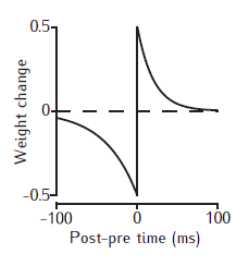
\includegraphics[width=.5\textwidth]{03_PlasticityInTheBrain/figures/pasted_image_6.png}
    \caption{STPD, spike timing dependent activity, graph if the post is active then per gave input no weight change (LTD) should occur. If the post fired then activated the pre then weight increased (LTP) should occur.}
    \label{fig:syn_plas1t}
\end{figure}

\begin{equation}
\begin{array}{l}
{\dot{w}=H(\text { pre, post })} \\
{\dot{w}=F(M, \text { pre, post })}
\end{array}
\end{equation}
    

Writing down hebbian learning it can be thought of as a H a function that detects the correlation of pre and postsynaptic potentials leading to a weight change. 

What was Geoffrey’s Problem with Hebbian Learning?
It isn’t error driven, in bp the neurons are trained so that everyone is optimised. These errors are important for hierarchical learning to gain correct responses. 

Multi Factor or neohebbain learning. 
The M acts as the third factor, it could be the error that allows it to become error driven. Biologists are examining this could be a global reward like dopamine or local activity. 


\subsubsection{Heterostatic Plasticity}
Is the modulation of the input into the post from the presynaptic neuron. This then leads to the change in the post either facilitatory with excitatory inputs or inhibitory with inhibitory inputs. 

Example Fly: neurons come into a brain area these act to modulate postsynaptic neurons. With greater activation the pre synatpic neurons grow irrespective of the postsynaptic activity.

Example 2: A the brain receives a reward it acts to modulate the synapse. It then changes the STDP profile it causes an increase in the synaptic strength irreseptic if the post or pre fires first. This is known as a Heterostatic Modulation.


\begin{figure}[H]
    \centering
    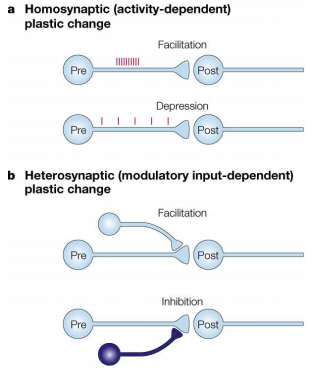
\includegraphics[width=.8\textwidth]{03_PlasticityInTheBrain/figures/pasted_image_8.png}
    \caption{Heterostatic Plasticity}
    \label{fig:syn_plas1t}
\end{figure}





\subsubsection{Behavior time scale Plasticity}

STP and STD (short term depression and potentiation) this occurs in the short term memory seconds to minutes, LTD and LTP occurs between seconds to minutes. 
The longer time scales the formation of new synapses as result short term processes hours to months. 
Then the ultra long time scales is the structural changes in brain regions. Months to lifetime.



\subsubsection{Time scales of synaptic plasticity (short term, LTP/LTD)}
Short term plasticity, determined by the amount of nts present, Short term depression occurs as there are less nts present. The nts in the cleft are reabsorbed leading to a restocking of the nts in the neuron. 

Short term facilitation results as increasing spiking leads to more Ca ions within the cell, this results in a greater spiking. 


%---------------------------
\subsection{The Hippocampus as a model system to study neural plasticity}
Hippocampus is a model system of learning and memory. Important system in the storage of memory. Cells between Ca3 and CA1 are used to encode places. This has been shown in rat experiments with the morris water maze. MWM is when a mouse is placed in a drum of milky white water and the mouse must find the platform and it’s movement is tracked with a camera. Over time the mouse will learn where the platform is. If certain receptors important to LTP and LTD the mouse does not learn. It shows that the learning is dependant on synaptic plasticity and hippocampus.

\begin{figure}[H]
    \centering
    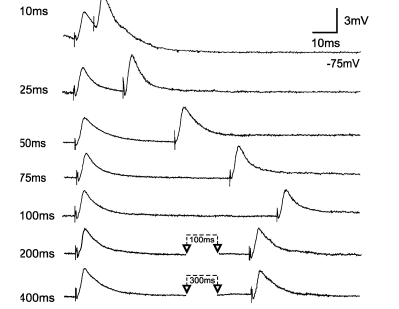
\includegraphics[width=.6\textwidth]{03_PlasticityInTheBrain/figures/pasted_image_9.png}
    \caption{Heterostatic Plasticity}
    \label{fig:syn_plas1t}
\end{figure}

\begin{figure}[H]
    \centering
    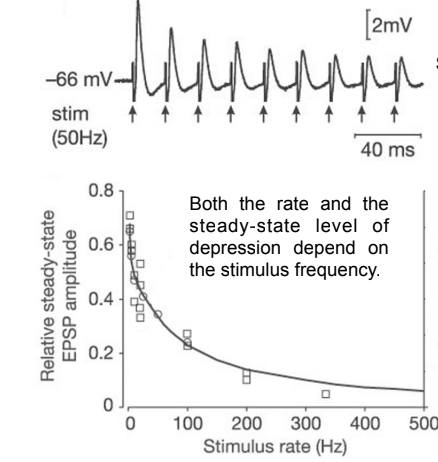
\includegraphics[width=.6\textwidth]{03_PlasticityInTheBrain/figures/pasted_image_10.png}
    \caption{Heterostatic Plasticity}
    \label{fig:syn_plas1t}
\end{figure}

To test plasticity in the hippocampus the Ca3 to Ca1 pathway was modulated and the EPSP in the Ca1 was measured, this tells you the activity of the pathway. If the spiked generated overlap it leads to increased spiking strength as there is Residual Ca2+ in the cell. Short term facilitation. Short term depression at about 40ms time frame can be observed if the CA3 to CA1 pathway is stimulated at 50 hz it leads to a reduction in the EPSP which dependant on the frequency of activation.

\begin{figure}[H]
    \centering
    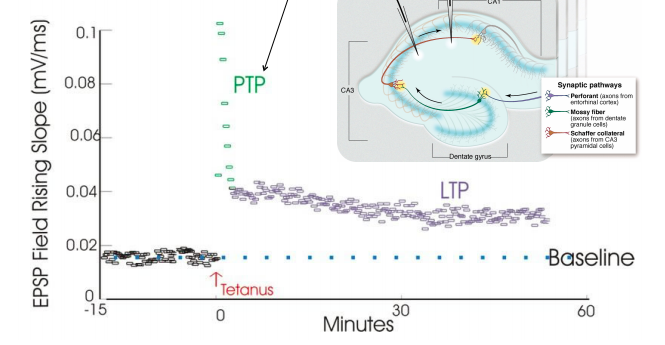
\includegraphics[width=.8\textwidth]{03_PlasticityInTheBrain/figures/pasted_image_11.png}
    \caption{Heterostatic Plasticity}
    \label{fig:syn_plas1t}
\end{figure}


LTP is measure in the hippocampus. The CA3 pathway is given a fast stimulus of (range of 50 - 200) 100 hz known as tetanus. This then leads to a stronger post tetanic potentiation caused by the accumulation of Ca in the terminals as well as LTP in the long term. If the cells are stimulated at a lower time frequency 1-10 hz LTD will occur. 




\subsubsection{LTP and LTD induction in the Hippocampus}
\subsubsection{Molecular basis of synaptic plasticity}

\begin{figure}[H]
    \centering
    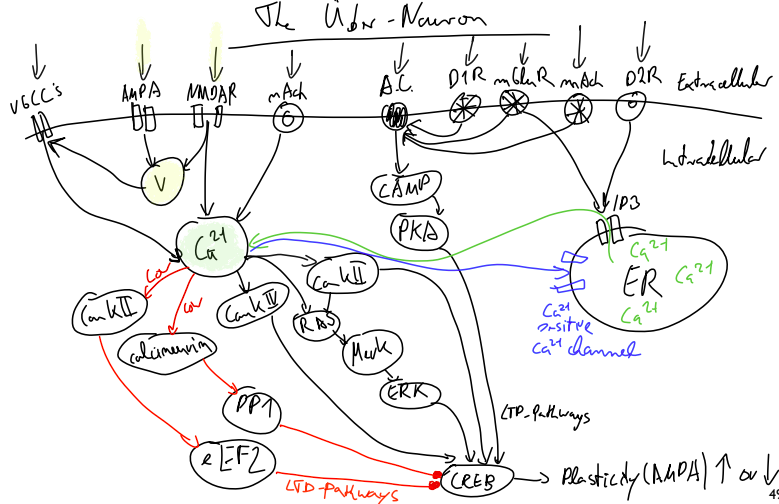
\includegraphics[width=.8\textwidth]{03_PlasticityInTheBrain/figures/pasted_image_12.png}
    \caption{}
    \label{fig:syn_plas1t}
\end{figure}

\paragraph{Intro}
Very simply LTP and LTD are dependent on CREB which controls the level of AMPA receptors in the cell. The level of AMPA receptors will determine how depolarised or hyperpolarised the cell becomes. 

\paragraph{What controls LTP and LTD:}
\begin{itemize}
    \item Creb is controlled by many pathways that are dependant on Ca ions or directly by dopamine. 
    \item Ca ion levels can increase as it enters into the cell from the external environment or released from internal stores.
\end{itemize}

\paragraph{How CA levels change:}
AMPA channel, when glutamate binds it causes depolarisation opening voltage gated Ca channels as well as NMDA channels that further depolarise the cells. 
Dopamine D2 when binds in leads to Ca2+ increase from the ER, this increased Ca leads. 

\paragraph{How CA leads to CREB:}
\begin{itemize}
    \item Positive: High levels of Ca activated Camkinse 1 and 2 that leads to increased Creb and thus ampa receptors. Dopamine activated internal cell machinery that leads to increased phosphorylation (activation) of creb these both pathways are known as the LTP pathways. 
    \item Negative: Low levels of Ca leads to Camkinse 2 and Calmodulin that reduces the phosphorylation (activation) of creb thus ampa receptors.
\end{itemize}

\paragraph{Summary}
Thus Ca is very important for LTP and LTD. Low frequency stimulation causes low Ca levels and high frequency leads to high levels.

%---------------------------
\subsection{Non-synaptic plasticity}
Researchers have artificially raised the Neuronal excitability below threshold. It leads to a greater number of firings. 

Researchers can modulate the axons with glutamate puffs and this will affect the action potential traveling along the axon. 

Researchers can modulate dendritic excitability 
If the volume is smaller the epsp will summed up leading to ap, the synapse location will also modulate the excitability nearer the soma will be more excitable as there isn’t a loss of charge.

\subsubsection{Neuronal excitability and spike generation}
\subsubsection{Axonal modulation (shunting, frequency filtering)}
\subsubsection{Alterations of dendritic excitability}


\subsection{QUIZ}
\begin{itemize}
    \item What are the differences between the weights of a deep network and the connections between biological neurons?: 
    In deep learning the weights are binary, if a neuron is activity it causes a change in the next layer.
    In biology if the action potential is modulated (axonal by myelinated and other factors) it will determine if the post neuron is activated, the dendritic epsp can be modulated before it reaches the axon hillock by summation and inhibition signals, the cell can in a refractory period or in excitability this means the effective connective between neurons can be modulated, also the inhibitory nts can modulate the epsp.
    \item Is synaptic plasticity the only mechanism that neurons can use to alter their effective connectivity?
    \item Is weight tuning by BP the only mechanism in DNNs that affect the weights?
\end{itemize}

\end{document}